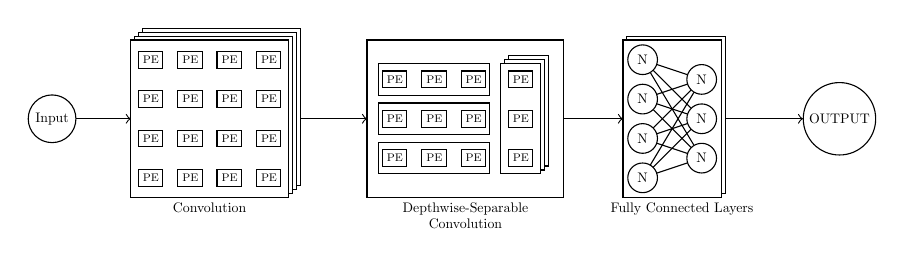
\begin{tikzpicture}[
	scale=0.5, transform shape,
	endpoint/.style = {
		circle, draw
	},
	pe/.style = {
		rectangle, draw,
		align=center,
		text width=11pt,
		font=\footnotesize
	},
	neuron/.style = {
		circle, draw,
		align=center,
		text width=10pt
	},
	label/.style = {
		anchor=north,
		align=center,
		text width=4cm
	}
]
	\node[endpoint] (in) at (0, 0) {Input};
	% Convolution Engine
	\node[label] at (4, -2) {Convolution};
	\foreach \i in {3,...,0} {
		\draw[fill=white] ({2 + \i/10}, {-2 + \i/10})
			rectangle ++(4, 4);
	}
	\foreach \x in {2,...,5} {
		\foreach \y in {-2,...,1} {
			\node[pe] at ({\x+0.5}, {\y+0.5}) {PE};
		}
	}
	% DSCV Engine
	\node[label] at (10.5, -2) {Depthwise-Separable Convolution};
	\draw[fill=white] (8, -2) rectangle ++(5, 4);
	% Depthwise
	\foreach \y in {-2,...,0} {
		\draw (8.3, {\y+0.6}) rectangle ++(2.8, 0.8);
		\foreach \x in {8,...,10} {
			\node[pe] at ({\x+0.7}, {\y+1}) {PE};
		}
	}
	% Pointwise
	\foreach \i in {2,...,0} {
		\draw[fill=white] ({11.4 + \i/10}, {-1.4 + \i/10})
			rectangle ++(1, 2.8);
	}
	\foreach \y in {-2,...,0} {
		\node[pe] at (11.9, {\y+1}) {PE};
	}
	% FC Layers
	\node[label] at (16, -2) {Fully Connected Layers};
	\foreach \i in {1,...,0} {
		\draw[fill=white] ({14.5 + \i/10}, {-2 + \i/10})
			rectangle ++(2.5, 4);
	}
	\node[neuron] (fc1a) at (15, -1.5) {N};
	\node[neuron] (fc1b) at (15, -0.5) {N};
	\node[neuron] (fc1c) at (15, 0.5) {N};
	\node[neuron] (fc1d) at (15, 1.5) {N};
	\node[neuron] (fc2a) at (16.5, -1) {N};
	\node[neuron] (fc2b) at (16.5, -0) {N};
	\node[neuron] (fc2c) at (16.5, 1) {N};
	\draw (fc1a) -- (fc2a);
	\draw (fc1b) -- (fc2a);
	\draw (fc1c) -- (fc2a);
	\draw (fc1d) -- (fc2a);
	\draw (fc1a) -- (fc2b);
	\draw (fc1b) -- (fc2b);
	\draw (fc1c) -- (fc2b);
	\draw (fc1d) -- (fc2b);
	\draw (fc1a) -- (fc2c);
	\draw (fc1b) -- (fc2c);
	\draw (fc1c) -- (fc2c);
	\draw (fc1d) -- (fc2c);
	%
	\node[endpoint] (out) at (20, 0) {OUTPUT};
	% Stage connections
	\draw[->] (in) -- ++(2, 0);
	\draw[->] (6.3, 0) -- ++(1.7, 0);
	\draw[->] (13, 0) -- ++(1.5, 0);
	\draw[->] (17.1, 0) -- (out);
\end{tikzpicture}
